\chapter{Long Short-Term Memory (LSTM) (1997)}

\begin{figure}[H]
    \centering
    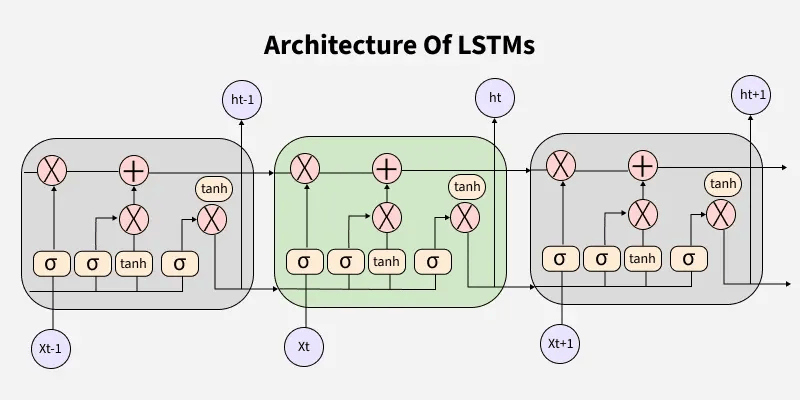
\includegraphics[
        width=\linewidth,
        height=6cm,
        keepaspectratio,
    ]{images/recurrent-neural-networks/lstm-gfg.chain-of-lstms.png}
    \caption{LSTM: unrolling \cite{geeksforgeeks/deep-learning/deep-learning-introduction-to-long-short-term-memory}}
\end{figure}


\begin{enumerate}
    \item Long Short-Term Memory (LSTM) is an \textbf{enhanced version} of the Recurrent Neural Network (RNN) designed by Hochreiter and Schmidhuber. 
    \hfill \cite{geeksforgeeks/deep-learning/deep-learning-introduction-to-long-short-term-memory}

    \item LSTMs can capture long-term dependencies in sequential data making them ideal for tasks like language translation, speech recognition and time series forecasting.
    \hfill \cite{geeksforgeeks/deep-learning/deep-learning-introduction-to-long-short-term-memory}

    \item Unlike traditional RNNs which use a single hidden state passed through time LSTMs introduce a \textbf{memory cell} that holds information over extended periods addressing the challenge of learning long-term dependencies.
    \hfill \cite{geeksforgeeks/deep-learning/deep-learning-introduction-to-long-short-term-memory}

    \item \textbf{Architecture}: LSTM architectures involves the memory cell which is controlled by three gates:
    \hfill \cite{geeksforgeeks/deep-learning/deep-learning-introduction-to-long-short-term-memory}
    \begin{enumerate}
        \item \textbf{Input gate}: Controls what information is added to the memory cell.
        \hfill \cite{geeksforgeeks/deep-learning/deep-learning-introduction-to-long-short-term-memory}
    
        \item \textbf{Forget gate}: Determines what information is removed from the memory cell.
        \hfill \cite{geeksforgeeks/deep-learning/deep-learning-introduction-to-long-short-term-memory}
    
        \item \textbf{Output gate}: Controls what information is output from the memory cell.
        \hfill \cite{geeksforgeeks/deep-learning/deep-learning-introduction-to-long-short-term-memory}
    \end{enumerate}
    This allows LSTM networks to selectively retain or discard information as it flows through the network which allows them to learn long-term dependencies. 
    The network has a hidden state which is like its \textbf{short-term memory}. 
    This memory is updated using the current input, the previous hidden state and the current state of the memory cell.
    \hfill \cite{geeksforgeeks/deep-learning/deep-learning-introduction-to-long-short-term-memory}
\end{enumerate}



\section{Working of LSTM}

\begin{figure}[H]
    \centering
    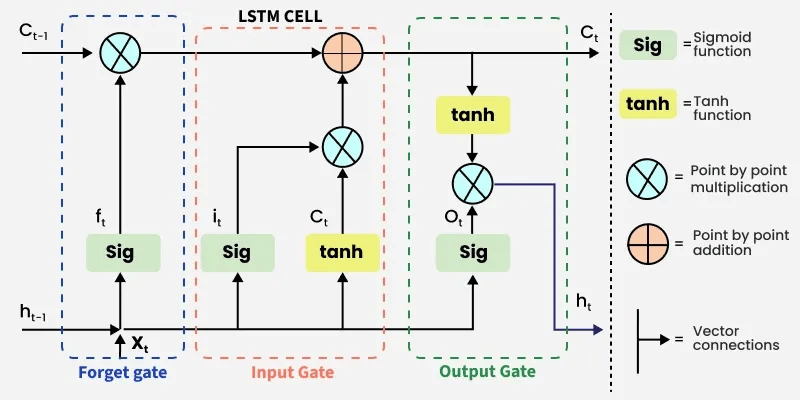
\includegraphics[
        width=\linewidth,
        height=6cm,
        keepaspectratio,
    ]{images/recurrent-neural-networks/lstm-gfg.fig-1.arch.png}
    \caption{
        LSTM Model 
        \cite{geeksforgeeks/deep-learning/deep-learning-introduction-to-long-short-term-memory}
    }
\end{figure}



\begin{lstlisting}[
    language=Python,
    caption=LSTM from scratch (PyTorch) \cite{common/online/chatgpt}
]
class ManualLSTM(nn.Module):
    def __init__(self, input_size, hidden_size, output_size):
        """
        Single-layer LSTM implemented without using nn.LSTM / nn.LSTMCell.
        Uses concatenated matrices for input-to-gates and hidden-to-gates:
          gates = x @ Wx + h @ Wh + b
        where gates are concatenation [i | f | g | o] (input, forget, cell, output)
        """
        super().__init__()
        self.input_size = input_size
        self.hidden_size = hidden_size

        # input -> gates (4 * hidden)
        self.Wx = nn.Parameter(torch.randn(input_size, 4 * hidden_size) * 0.1)
        # hidden -> gates (4 * hidden)
        self.Wh = nn.Parameter(torch.randn(hidden_size, 4 * hidden_size) * 0.1)
        # bias (4 * hidden)
        self.b = nn.Parameter(torch.zeros(4 * hidden_size))

        # final classifier from last hidden state
        self.Why = nn.Parameter(torch.randn(hidden_size, output_size) * 0.1)
        self.by = nn.Parameter(torch.zeros(output_size))

    def forward(self, x, h0=None, c0=None):
        """
        x: (batch, seq_len, input_size)
        returns logits (batch, output_size) and (h_last, c_last)
        """
        batch, seq_len, _ = x.shape
        H = self.hidden_size

        if h0 is None:
            h = x.new_zeros(batch, H)
        else:
            h = h0
        if c0 is None:
            c = x.new_zeros(batch, H)
        else:
            c = c0

        for t in range(seq_len):
            xt = x[:, t, :]  # (batch, input_size)
            gates = xt @ self.Wx + h @ self.Wh + self.b  # (batch, 4*H)
            # split gates into i, f, g, o
            i, f, g, o = gates.chunk(4, dim=1)
            i = torch.sigmoid(i)
            f = torch.sigmoid(f)
            g = torch.tanh(g)         # candidate cell
            o = torch.sigmoid(o)

            c = f * c + i * g
            h = o * torch.tanh(c)

        logits = h @ self.Why + self.by  # (batch, output_size)
        return logits, (h, c)
\end{lstlisting}



\subsection{Forget Gate}

\begin{enumerate}
    \item The information that is no longer useful in the cell state is removed with the forget gate.
    \hfill \cite{geeksforgeeks/deep-learning/deep-learning-introduction-to-long-short-term-memory}

    \item Two inputs $x_t$ (input at the particular time) and $h_{t-1}$ (previous cell output) are fed to the gate and multiplied with weight matrices followed by the addition of bias. 
    The resultant is passed through \textbf{sigmoid activation function} which gives output in range of $[0,1]$. 
    \hfill \cite{geeksforgeeks/deep-learning/deep-learning-introduction-to-long-short-term-memory}
    
    \item If for a particular cell state the output is $0$ or near to $0$, the piece of information is \textbf{forgotten} and for output of $1$ or near to $1$, the information is \textbf{retained} for future use. 
    \hfill \cite{geeksforgeeks/deep-learning/deep-learning-introduction-to-long-short-term-memory}

    \item \colorbox{yellow}{$ f_t=\sigma(W_f\cdot[h_{t-1},x_t]+b_f) $}
    \hfill \cite{geeksforgeeks/deep-learning/deep-learning-introduction-to-long-short-term-memory}
    \begin{enumerate}
        \item $W_f$ represents the weight matrix associated with the forget gate.
        \hfill \cite{geeksforgeeks/deep-learning/deep-learning-introduction-to-long-short-term-memory}

        \item $[h_{t-1},x_t]$ denotes the concatenation of the current input and the previous hidden state.
        \hfill \cite{geeksforgeeks/deep-learning/deep-learning-introduction-to-long-short-term-memory}

        \item $b_f$ bias with the forget gate
        \hfill \cite{geeksforgeeks/deep-learning/deep-learning-introduction-to-long-short-term-memory}

        \item $\sigma$ sigmoid activation function
        \hfill \cite{geeksforgeeks/deep-learning/deep-learning-introduction-to-long-short-term-memory}
    \end{enumerate}
\end{enumerate}


\subsection{Input gate}

\begin{enumerate}
    \item The addition of useful information to the cell state is done by the input gate.
    \hfill \cite{geeksforgeeks/deep-learning/deep-learning-introduction-to-long-short-term-memory}

    \item First the information is regulated using the \textbf{sigmoid function} and filter the values to be remembered similar to the forget gate using inputs $h_{t-1}$ and $x_t$. 
    \hfill \cite{geeksforgeeks/deep-learning/deep-learning-introduction-to-long-short-term-memory}
    \\[0.2cm]
    .\hfill
    \colorbox{yellow}{$ i_t=\sigma(W_i\cdot [h_{t-1},x_t]+b_i) $}
    \hfill \cite{geeksforgeeks/deep-learning/deep-learning-introduction-to-long-short-term-memory}
    
    \item Then, a vector is created using $\bm{\tanh}$ \textbf{function} that gives an output from $-1$ to $+1$ which contains all the possible values from $h_{t-1}$ and $x_t$. 
    \hfill \cite{geeksforgeeks/deep-learning/deep-learning-introduction-to-long-short-term-memory}
    \\[0.2cm]
    .\hfill
    \colorbox{yellow}{$ \hat{C}_t=\tanh(W_c\cdot[h_{t-1},x_t]+b_c) $}
    \hfill \cite{geeksforgeeks/deep-learning/deep-learning-introduction-to-long-short-term-memory}
    
    \item At last the values of the vector and the regulated values are multiplied to obtain the useful information. 
    \hfill \cite{geeksforgeeks/deep-learning/deep-learning-introduction-to-long-short-term-memory}

    \item We multiply the previous state by $f_t$ effectively filtering out the information we had decided to ignore earlier. 
    Then we add $i_t \odot C_t$ which represents the new \textbf{candidate} values scaled by how much we decided to update each state value.
    \hfill \cite{geeksforgeeks/deep-learning/deep-learning-introduction-to-long-short-term-memory}
    \\[0.2cm]
    .\hfill
    \colorbox{yellow}{$ C_t=f_t \odot C_{t-1}+i_t \odot \hat{C}_t $}
    \hfill \cite{geeksforgeeks/deep-learning/deep-learning-introduction-to-long-short-term-memory}

    \item $\odot$ denotes element-wise multiplication
    \hfill \cite{geeksforgeeks/deep-learning/deep-learning-introduction-to-long-short-term-memory}

    \item $\tanh$ is activation function
    \hfill \cite{geeksforgeeks/deep-learning/deep-learning-introduction-to-long-short-term-memory}
\end{enumerate}





\subsection{Output gate}

\begin{enumerate}
    \item The output gate is responsible for deciding what part of the current cell state should be sent as the hidden state (output) for this time step.
    \hfill \cite{geeksforgeeks/deep-learning/deep-learning-introduction-to-long-short-term-memory}

    \item First, the gate uses a \textbf{sigmoid function} to determine which information from the current cell state will be output. 
    This is done using the previous hidden state $h_{t-1}$ and the current input $x_t$:
    \hfill \cite{geeksforgeeks/deep-learning/deep-learning-introduction-to-long-short-term-memory}
    \\[0.2cm]
    .\hfill
    \colorbox{yellow}{$o_t=\sigma(W_o\cdot[h_{t-1},x_t]+b_o)$}
    \hfill \cite{geeksforgeeks/deep-learning/deep-learning-introduction-to-long-short-term-memory}

    \item Next, the current cell state $C_t$ is passed through a tanh activation to scale its values between $-1$ and $+1$. 
    Finally, this transformed cell state is multiplied element-wise with $o_t$ to produce the hidden state $h_t$:
    \hfill \cite{geeksforgeeks/deep-learning/deep-learning-introduction-to-long-short-term-memory}
    \\[0.2cm]
    .\hfill
    \colorbox{yellow}{$ h_t=o_t\odot\tanh(C_t) $}
    \hfill \cite{geeksforgeeks/deep-learning/deep-learning-introduction-to-long-short-term-memory}
    \\[0.2cm]
    This hidden state $h_t$ is then passed to the next time step and can also be used for generating the output of the network.
    \hfill \cite{geeksforgeeks/deep-learning/deep-learning-introduction-to-long-short-term-memory}

    \begin{enumerate}
        \item $o_t$ is the output gate activation.
        \hfill \cite{geeksforgeeks/deep-learning/deep-learning-introduction-to-long-short-term-memory}
        
        \item $C_t$ is the current cell state.
        \hfill \cite{geeksforgeeks/deep-learning/deep-learning-introduction-to-long-short-term-memory}
        
        \item $\odot$ represents element-wise multiplication.
        \hfill \cite{geeksforgeeks/deep-learning/deep-learning-introduction-to-long-short-term-memory}
        
        \item $\sigma$ is the sigmoid activation function.
        \hfill \cite{geeksforgeeks/deep-learning/deep-learning-introduction-to-long-short-term-memory}
    \end{enumerate}

\end{enumerate}








